\chapter*{\RL{ملخص}}
% \chapter*{ملخص}

\addcontentsline{toc}{chapter}{Résumé en Arabe}


% \Huge
% \begin{RLtext}
%     \bigskip
%     ملخص
% \end{RLtext}
% 
\includegraphics[scale=22]{Images/ملخص.png} % 
\includepdf[pages=-,fitpaper]{ملخص.pdf}
% 
\includepdf[pages=-]{ملخص.pdf}
\begin{center}
    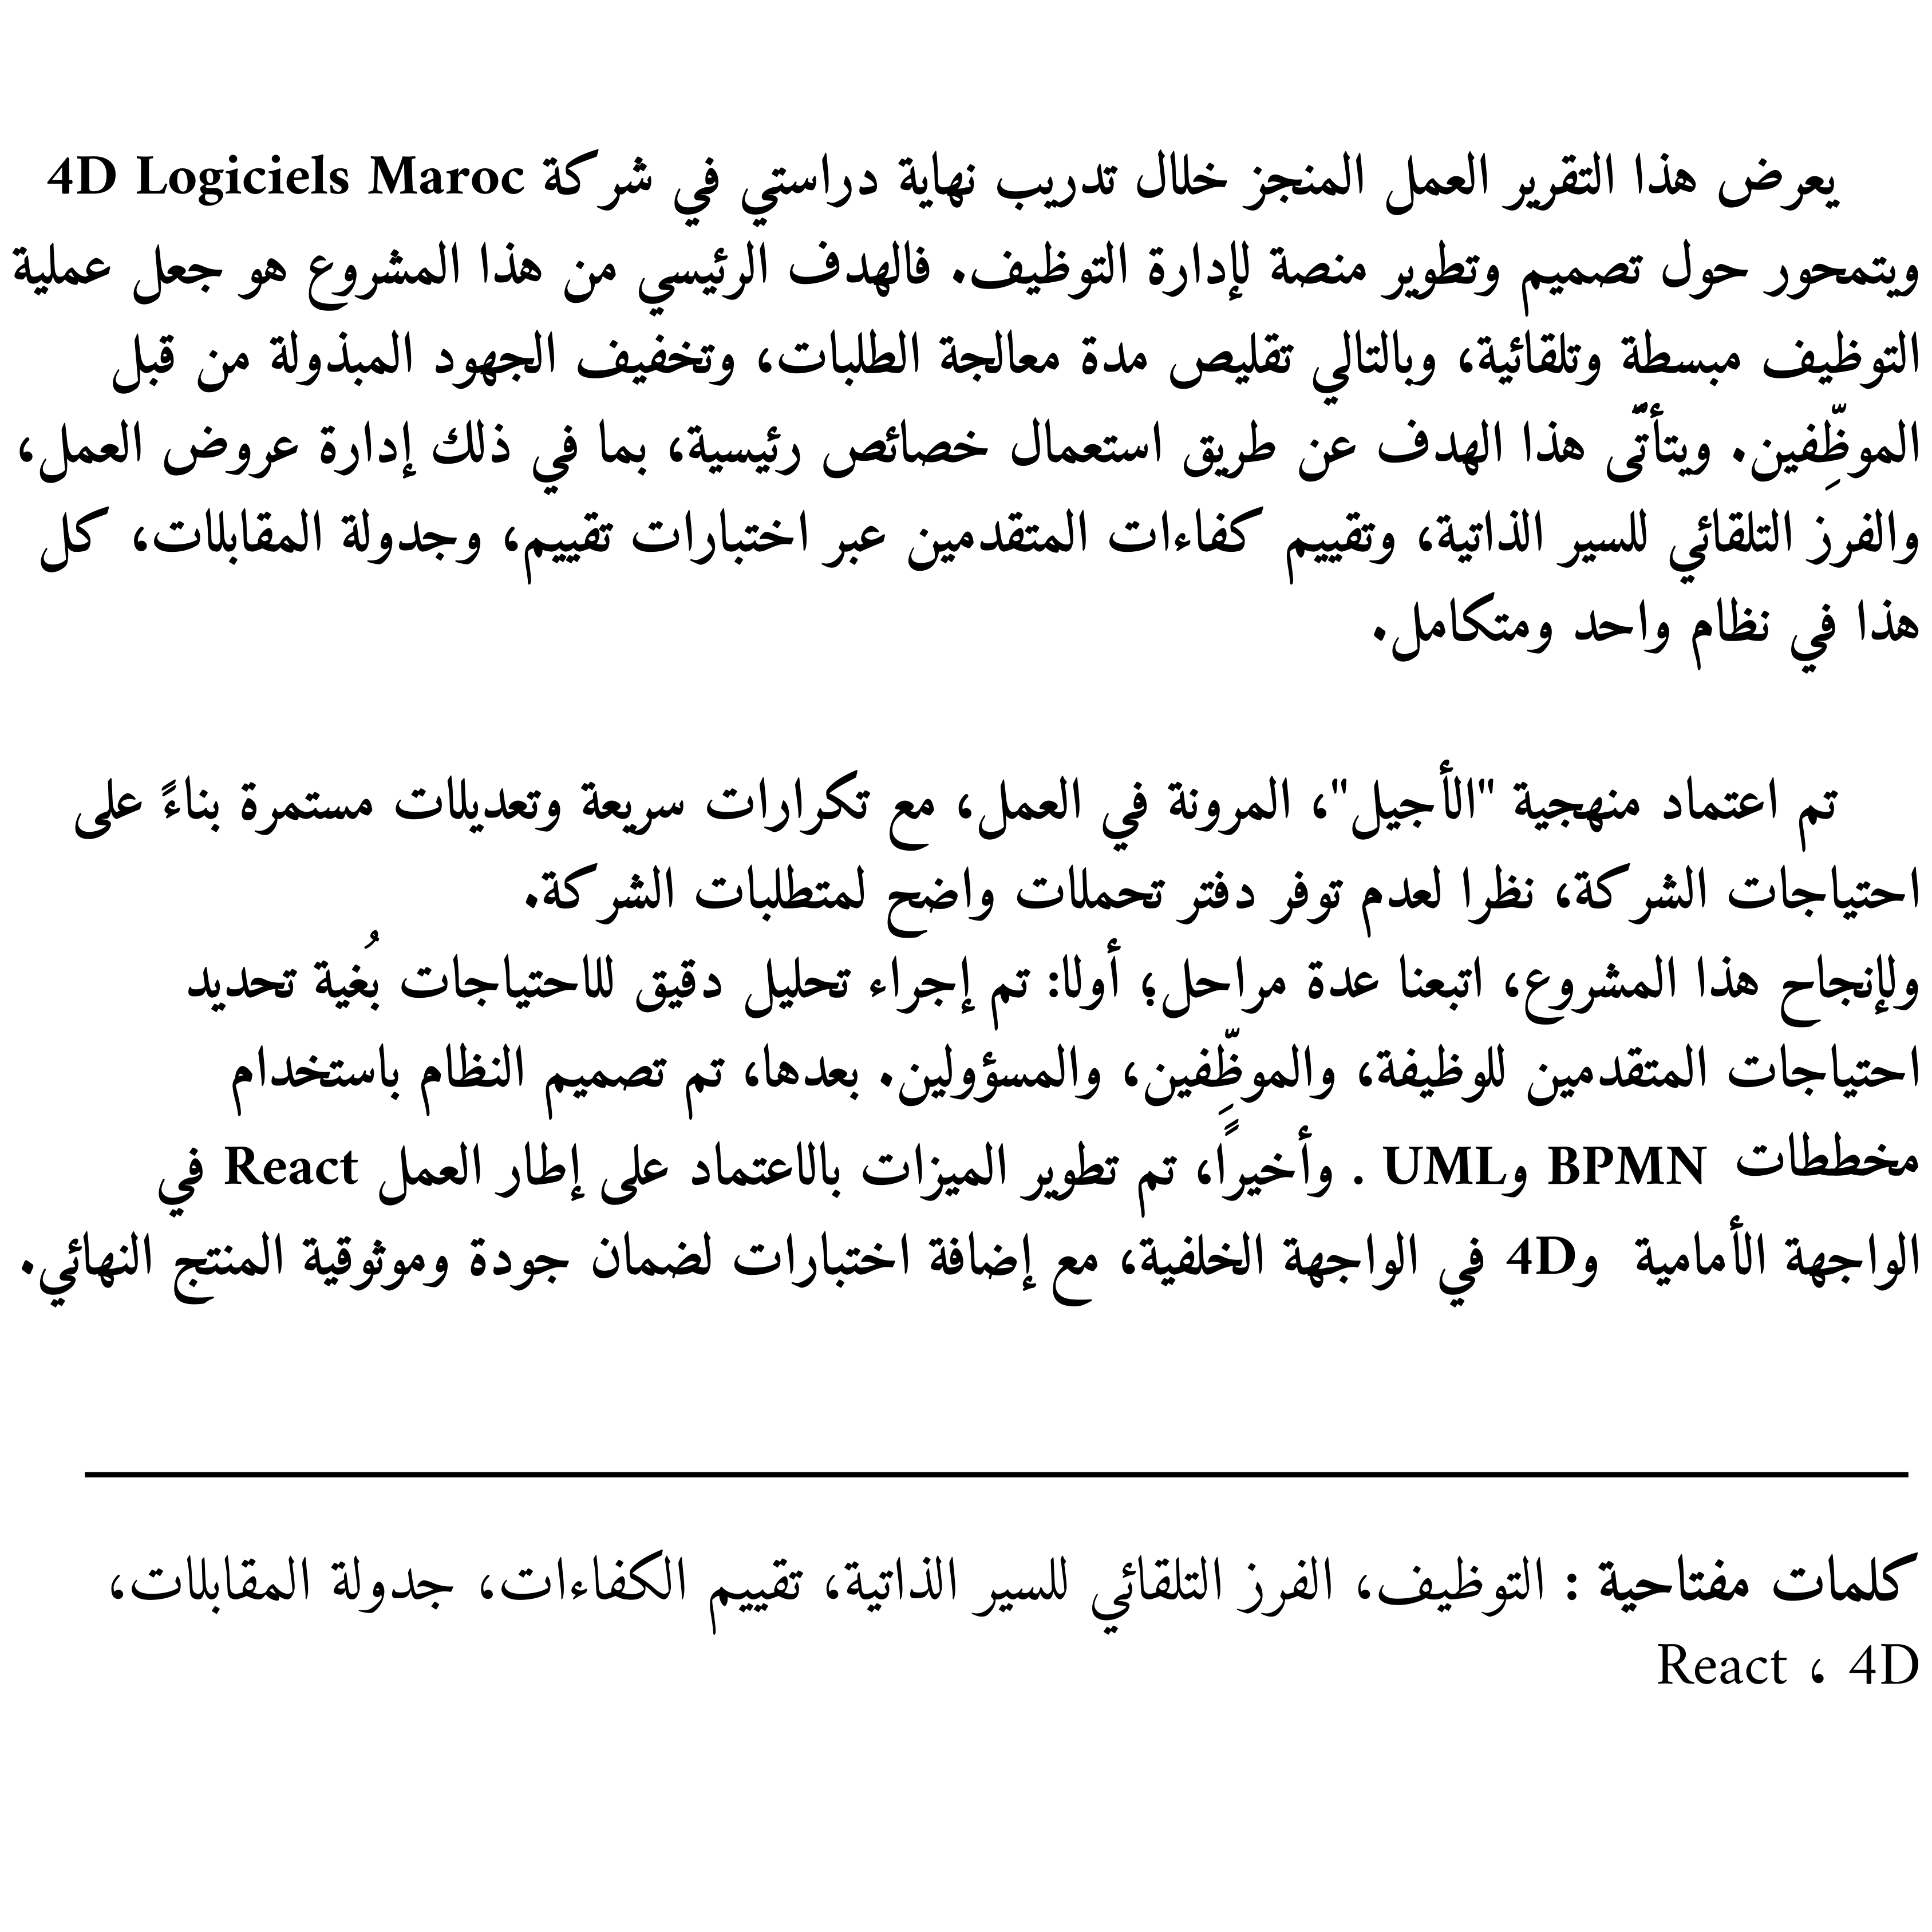
\includegraphics[width=\textwidth]{Images/molkhassss.png} % 
\includepdf[pages=-,fitpaper]{ملخص.pdf}    
\end{center}
% [width=\textwidth,height=\textheight,keepaspectratio]
% \begin{spacing}{1.25}
    
% \begin{RLtext}
% يقدم هذا التقرير العمل المنجز خلال فترة تدريبي النهائي في شركة 
% 4D Logiciels Maroc،
%  الذي يركز على تصميم وتطوير منصة لإدارة التوظيف. الهدف الرئيسي من هذا المشروع هو تبسيط وأتمتة عملية التوظيف، وبالتالي تقليل أوقات معالجة الطلبات والجهود المبذولة من قبل المجندين. سيتم تحقيق ذلك عن طريق دمج ميزات رئيسية، بما في ذلك إدارة عروض العمل، الفرز التلقائي للسير الذاتية، تقييم كفاءات المتقدمين من خلال اختبارات التقييم، وجدولة المقابلات في نظام متكامل.
% \end{RLtext}
% \vspace{0.7cm}

% \begin{RLtext}
% تم اعتماد منهجية الأجايل، مع تكرارات سريعة وتعديلات مستمرة بناءً على الاحتياجات، نظراً لعدم وجود وثيقة محددة للمتطلبات.
% \end{RLtext}
% \vspace{0.7cm}


% \begin{RLtext}
% لإتمام هذا المشروع، اتبعنا عدة مراحل. أولاً، تم إجراء تحليل دقيق للاحتياجات لتحديد متطلبات المتقدمين، المجندين، والمسؤولين. بعد ذلك، تم تصميم النظام باستخدام مخططات UML وBPMN. وأخيراً، تم تطوير الميزات بناءً على إطار عمل 4D في الجانب الخلفي، مع دمج اختبارات لضمان جودة وموثوقية المنتج النهائي.
% \end{RLtext}

% \end{spacing}
% \vspace{0.7cm}

% \noindent\rule[2pt]{\textwidth}{0.5pt}

% \begin{RLtext} 

% {\textbf{الكلمات المفتاحية}}

% التوظيف، الفرز التلقائي للسير الذاتية، تقييم الكفاءات، جدولة المقابلات
% \\

% \end{RLtext}

